%░▒█▀▀▀█░▒█▀▀▀░▒█▀▀▄░▒█▀▄▀█░░░▒█▀▀▄░▒█▀▀▀░▒█░░▒█░▀█▀░▒█▀▀▀░▒█░░▒█
%░▒█░░▒█░▒█▀▀░░▒█░▒█░▒█▒█▒█░░░▒█▄▄▀░▒█▀▀▀░░▒█▒█░░▒█░░▒█▀▀▀░▒█▒█▒█
%░▒█▄▄▄█░▒█░░░░▒█▄▄█░▒█░░▒█░░░▒█░▒█░▒█▄▄▄░░░▀▄▀░░▄█▄░▒█▄▄▄░▒▀▄▀▄▀
%.:..:..:..:..:..:..:..:..:..:..:..:..:..:..:..:..:..:..:..:.
\section{Orthogonal Frequency Division Multiplexing}

\gls{OFDM} is a modulation technique widely used in high speed wireless communication systems. It divides a channel into a number of equally spaced frequency bands.

%~^~~^~~^~~^~~^~~^~~^~~^~~^~~^~~^~~^~~^~~^~~^~~^~~^~~^~~^~~^~
\subsection{The History of OFDM}
\gls{MCM} was initially used for military \gls{HF} radios in the years 1950--1960. The use of orthogonal frequencies for transmission first appears in a 1966 patent by \emph{Robert W. Chang} of Bell Laboratories\cite{ofdm_intro}.
The proposal to use \gls{FFT} to generate orthogonal signals originally surfaced in 1969. Parallel data streams and \gls{FDM} would be used, but with overlapping sub-channels. The merits of this method include:
\begin{itemize}
	\item Avoiding the use of high speed equalization.
	\item Mitigation of impulsive noise and multi-path distortion.
	\item Maximal utilization of available bandwidth.
\end{itemize}
The earliest adoption of OFDM is seen in military communication.
\begin{figure}[!ht]
	\centering
	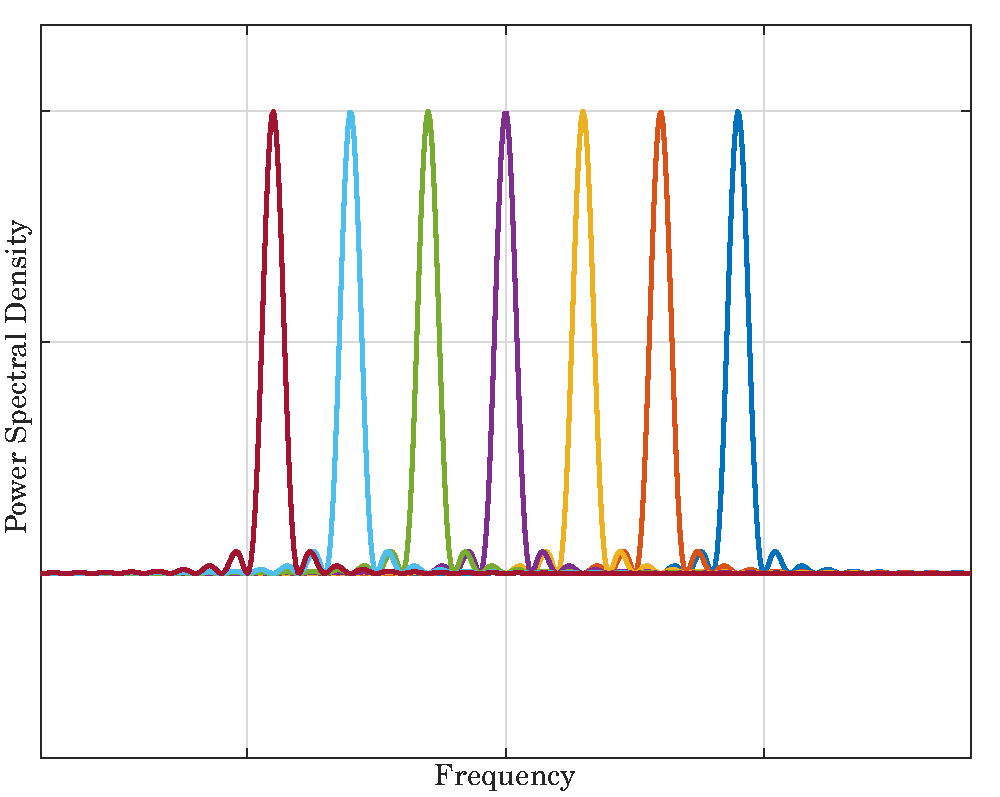
\includegraphics[width=0.8\textwidth]{Graphics/LiteratureReview/fdm.pdf}
	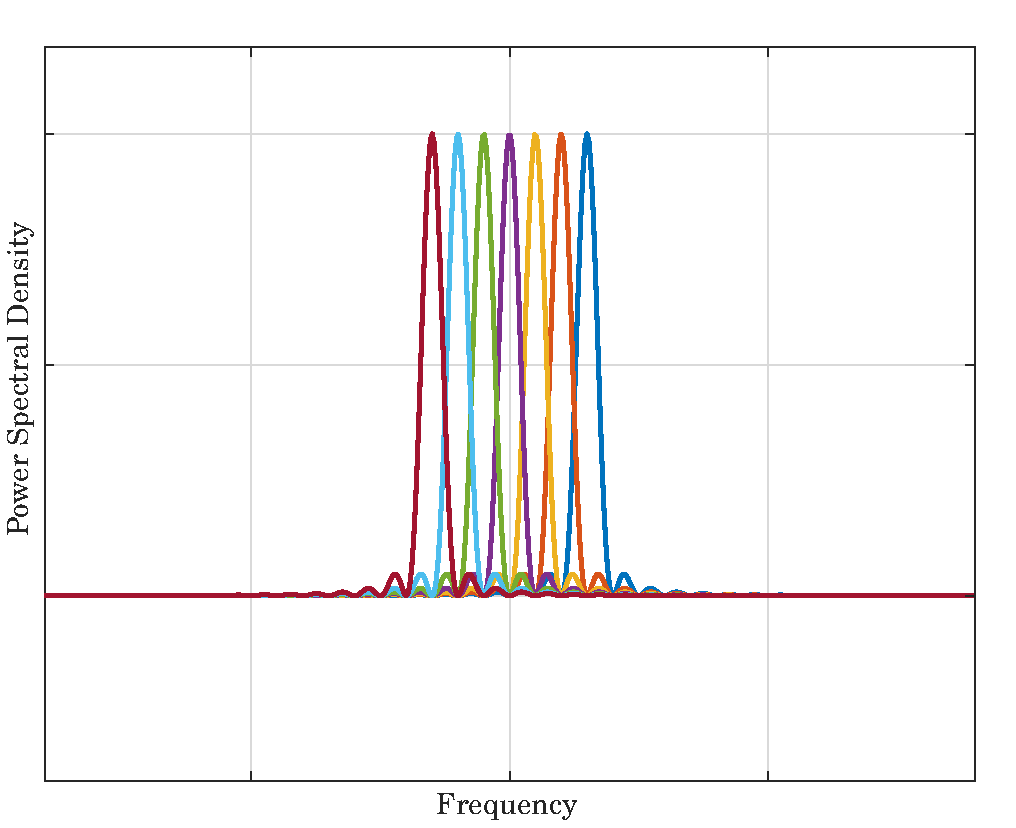
\includegraphics[width=0.8\textwidth]{Graphics/LiteratureReview/ofdmPSD.pdf}
	\caption{Comparison of OFDM and FDM spectral utilization}
	\label{fig:litRev:fdm}
\end{figure}

Thereafter, some fundamental improvements were incorporated into OFDM, most notably the inclusion of a \emph{cyclic prefix} in the early 1980s. The technique started to be considered for practical adoption in the mid 80s. In 1987, particularly, \emph{Lassalle} and \emph{Alard}, based in France, considered the use of OFDM for radio broadcasting. They noted the necessity of combining \gls{FEC} with \gls{OFDM}.

A novel application of OFDM was pioneered by \emph{Cioffi} and others at \emph{Stanford}, who showed its potential as a modulation technique for \gls{DSL} applications. In 1999, the first OFDM \gls{WLAN} standard \emph{802.11a} was published, followed in succession by \emph{802.11n} and \emph{802.16d}. However, the most widely deployed \gls{WLAN} standard is \emph{802.11b}, which uses \gls{DSSS}. OFDM is the basis of many telecommunication standards.

%,-.,-.,-.,-.,-.,-.,-.,-.,-.,-.,-.,-.,-.,-.,-.,-.,-.,-.,-.,-.
\subsubsection{IEEE 802.11 Standard}
The \emph{IEEE 802.11} specification is a standard that specifies the set requirements for the physical layer and a medium access control layer. The standard provides two definitions for physical layers-- \emph{802.11b} for \SI{2.4}{\giga\hertz} operation and \emph{802.11a} for \SI{5}{\giga\hertz} operation\cite{802.11}.

\emph{802.11a} and \emph{802.11b} are not inter-operable unless the equipment in use has dual band capability. These are the standard's specifications:
\begin{table}
	\centering
	\renewcommand{\arraystretch}{1.5}
	\begin{tabular}{l l}
		\emph{Parameter} & \emph{Value}\\
		\hline
		Modulation technique & BPSK, QPSK, 16-QAM, 64-QAM \\
		Coding rate & 1/2, 2/3, 3/4 \\
		Number of subcarriers & 52 \\
		Number of pilots & 4 \\
		Symbol duration & \SI{4}{\micro\second} \\
		Guard interval & \SI{800}{\nano\second} \\
		Sub-carrier spacing & \SI{312.5}{\kilo\hertz} \\
		\SI{3}{\decibel} bandwidth & \SI{16.56}{\mega\hertz} \\
		Channel spacing & \SI{20}{\hertz}
	\end{tabular}
	\label{tab:litRev:802.11}
\end{table}
All data sub-carriers use the same modulation format within a given burst but this can vary from burst to burst.

%~^~~^~~^~~^~~^~~^~~^~~^~~^~~^~~^~~^~~^~~^~~^~~^~~^~~^~~^~~^~
\subsection{OFDM Variants}
Variants of OFDM follow the standard implementation but possess additional attributes. Some of these include:
%`'`'`'`'`'`'`'`'`'`'
\paragraph{Coded OFDM} This is a variant of OFDM in which error correcting code is incorporated into the signal.
%`'`'`'`'`'`'`'`'`'`'
\paragraph{Flash OFDM} This is a fast-hopped version of OFDM which utilized multiple tones and fast hopping to spread signals over a given spectrum band.
%`'`'`'`'`'`'`'`'`'`'
\paragraph{Vector OFDM} This variant uses \gls{MIMO} techniques. It is a proprietary variant being developed by CISCO Systems. \gls{MIMO} techniques involve the use of multiple antennas to transmit and receive such that multi-path effects can be utilized to enhance signal reception and transmission speeds.
%`'`'`'`'`'`'`'`'`'`'
\paragraph{Wideband OFDM} A form of OFDM that uses such a large degree of spacing between its sub-channels that frequency errors between transmitter and receiver do not affect communication performance. It is particularly applicable to Wi-Fi systems.

%~^~~^~~^~~^~~^~~^~~^~~^~~^~~^~~^~~^~~^~~^~~^~~^~~^~~^~~^~~^~
\subsection{Principles of OFDM}
\gls{OFDM} is a type of \gls{MCM}, with the most apparent advantage of being that simultaneous transmission of \(N\) symbols over \(N\) sub-carriers reduces symbol rate \(1/N\) times the original. This also means that symbol duration is increased \(N\) times, which extenuates \gls{ISI}, consequently reducing the need for channel equalization.

Recovering the signals of the sub-channels at the receiver can be achieved through:
\begin{itemize}
	\item Spacing sub-carrier frequencies such that the spectra of \(N\) sub-channels do not overlap. \(N\) \gls{BPF}s are then used to separate these sub-channels, each requiring a sharp frequency response. This is the method used in \gls{OFDM}.
	\item Allowing the sub-carriers which are orthogonally spaced by \(1/T\) to overlap. The signals in the sub-carriers are recovered from the sub-carriers using correlators in the receiver. This method is used in \gls{OFDM}.
\end{itemize}
The advantages of \gls{OFDM} over single carrier modulation are:
\begin{enumerate}
	\item The Nyquist's rate for a given channel can be approached without the use of sharp cutoff filters.
	\item It elongates symbol period, countering the effects of \gls{ISI} due to channel dispersion and multipath interference.
	\item OFDM divides the frequency band into narrow bands, reducing sensitivity to wide-band impulse noise and frequency selective fading. The complex fading coefficient on each sub-band signal can be removed by multiplying the signal with the conjugate of the fading coefficient.
	\item Different modulation formats can be used on different sub-carriers depending on sub-channel noise.
	\item OFDM is digitally implementable using \gls{IDFT}/\gls{DFT} pair through their \gls{IFFT}/\gls{FFT} algorithm pair, greatly reducing system complexity.
\end{enumerate}
Wide adoption of OFDM in recent years has been commensurate with increasing computing power.

%,-.,-.,-.,-.,-.,-.,-.,-.,-.,-.,-.,-.,-.,-.,-.,-.,-.,-.,-.,-.
\subsubsection{OFDM Signal and Spectrum}
The final form of an OFDM signal can be a \emph{baseband} or a \emph{bandpass} signal. It is always baseband for wired systems due to limited bandwidth. In wireless systems, baseband signals are up-converted to the \gls{RF} band for transmission.
%`'`'`'`'`'`'`'`'`'`'
\paragraph{Baseband OFDM Signal} Its general form is expressed as:
\begin{align*}
	s(t) &= \sum_{i=0}^{N-1}s_i(t) = \sum_{i=0}^{N-1}A_i \cos (2\pi f_i t + \phi_i) & 0 \leq t \leq T
\end{align*}
\begin{mathDef}
	\mathSymb{A_i}{Amplitude of \(i\)\textsuperscript{th} subcarrier}
	\mathSymb{f_i}{Frequency of \(i\)\textsuperscript{th} subcarrier}
	\mathSymb{\phi_i}{Phase of \(i\)\textsuperscript{th} subcarrier}
	\mathSymb{N}{Number of subcarriers}
	\mathSymb{T}{Symbol period of the data}
\end{mathDef}
Depending on the modulation format (\gls{ASK} or \gls{PSK}), \(A_i\) or \(\phi_i\) respectively are determined by data while the others remain constant.
%`'`'`'`'`'`'`'`'`'`'
\paragraph{Proof of orthogonality} For the sub-carriers to be orthogonal, \(f_i\) must be integer multiples of \(1/2T\) and the minimum frequency separation between them must be \(1/T\). The subcarrier frequencies are taken to be:
\begin{align}
	f_i &= iR_s = \frac{i}{T} & i = 0, 1, \ldots, N-1
\end{align}
\begin{mathDef}
	\mathSymb{R_s}{Symbol duration}
\end{mathDef}

